\section{Illustrative results}
\label{sec:resultados}

All numbers in this section are \textbf{generated automatically} by \texttt{npm run paper:figures} from the repository's \texttt{runSimulation} engine. Figures use \texttt{pgfplots} reading CSV files exported by the same script, so small parameter tweaks can be reflected quickly in the PDF.

% Gerado por scripts/generate-paper-figures.ts
\newcommand{\StatCompletedA}{7}
\newcommand{\StatMeanCtA}{2.71}
\newcommand{\StatMedianCtA}{3.00}
\newcommand{\StatCompletedB}{7}
\newcommand{\StatMeanCtB}{2.57}
\newcommand{\StatMedianCtB}{2.00}
\newcommand{\StatCompletedC}{7}
\newcommand{\StatMeanCtC}{3.00}
\newcommand{\StatMedianCtC}{3.00}
\newcommand{\StatCompletedD}{7}
\newcommand{\StatMeanCtD}{2.71}
\newcommand{\StatMedianCtD}{3.00}


Figure~\ref{fig:cfdA} shows queue dynamics in scenario A: how \texttt{backlog} stock relates to work in progress in the specialty columns. Figures~\ref{fig:bar} and~\ref{fig:tp} summarize cross-scenario comparisons: the first highlights mean cycle time (the median complements Table~\ref{tab:resumoCenarios}), while the second shows throughput differences per sprint when the pairwise synergy pattern changes.

\begin{figure}[htbp]
  \centering
  % Generated by scripts/generate-paper-figures.ts
\begin{tikzpicture}
\begin{axis}[
  width=0.95\linewidth,
  height=5.4cm,
  xmin=1,
  xlabel={Dia global},
  ylabel={Cartões por coluna},
  legend columns=3,
  legend style={font=\scriptsize,at={(0.5,1.02)},anchor=south},
]
\addplot[thick,const plot,color=black!70] table[col sep=comma,x=day,y=backlog]{data/cfd_A_baseline.csv};
\addplot[thick,const plot,color=violet!80] table[col sep=comma,x=day,y=analise]{data/cfd_A_baseline.csv};
\addplot[thick,const plot,color=teal!80] table[col sep=comma,x=day,y=dev]{data/cfd_A_baseline.csv};
\addplot[thick,const plot,color=orange!90] table[col sep=comma,x=day,y=teste]{data/cfd_A_baseline.csv};
\addplot[thick,const plot,color=red!80] table[col sep=comma,x=day,y=deploy]{data/cfd_A_baseline.csv};
\legend{Backlog,Análise,Dev,Testes,Deploy}
\end{axis}
\end{tikzpicture}

  \caption{Card counts per column over global days in scenario A (baseline).}
  \label{fig:cfdA}
\end{figure}

\begin{figure}[htbp]
  \centering
  % Generated by scripts/generate-paper-figures.ts
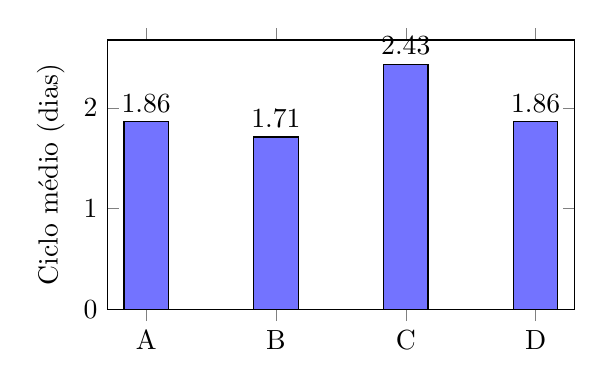
\begin{tikzpicture}
\begin{axis}[
  width=0.62\linewidth,
  height=5cm,
  ybar,
  ymin=0,
  symbolic x coords={A,B,C,D},
  xtick=data,
  xticklabel style={align=center},
  ylabel={Ciclo médio (dias)},
  nodes near coords,
  nodes near coords align={vertical},
  bar width=16pt,
]
\addplot[fill=blue!55] coordinates {(A,1.86) (B,1.71) (C,2.43) (D,1.86)};
\end{axis}
\end{tikzpicture}

  \caption{Mean cycle time (days) per scenario, considering only cards completed in the simulated window.}
  \label{fig:bar}
\end{figure}

\begin{figure}[htbp]
  \centering
  % Generated by scripts/generate-paper-figures.ts
\begin{tikzpicture}
\begin{axis}[
  width=0.95\linewidth,
  height=5.2cm,
  xlabel={Sprint},
  ylabel={Cartões concluídos},
  xmin=1,
  xmax=10,
  ymin=0,
  legend style={font=\scriptsize,at={(0.5,1.02)},anchor=south},
  legend columns=4,
]
\addplot[thick,mark=*,color=black!70] table[col sep=comma,x=sprint,y=A]{data/throughput_by_sprint.csv};
\addplot[thick,mark=square*,color=blue!70] table[col sep=comma,x=sprint,y=B]{data/throughput_by_sprint.csv};
\addplot[thick,mark=triangle*,color=red!75] table[col sep=comma,x=sprint,y=C]{data/throughput_by_sprint.csv};
\addplot[thick,mark=diamond*,color=teal!80] table[col sep=comma,x=sprint,y=D]{data/throughput_by_sprint.csv};
\legend{A,B,C,D}
\end{axis}
\end{tikzpicture}

  \caption{Throughput per sprint (cards reaching \texttt{deploy} in that sprint) for the four scenarios.}
  \label{fig:tp}
\end{figure}

\begin{table}[htbp]
  \centering
  \caption{Summary of the four scenarios (mean and median cycle in days; values generated in \texttt{summary\_stats.tex}).}
  \label{tab:resumoCenarios}
  \begin{tabular}{@{}lccc@{}}
    \toprule
    Scenario & Completed & Mean cycle & Median cycle \\
    \midrule
    A & \StatCompletedA & \StatMeanCtA & \StatMedianCtA \\
    B & \StatCompletedB & \StatMeanCtB & \StatMedianCtB \\
    C & \StatCompletedC & \StatMeanCtC & \StatMedianCtC \\
    D & \StatCompletedD & \StatMeanCtD & \StatMedianCtD \\
    \bottomrule
  \end{tabular}
\end{table}

\paragraph{Quick read.}
In the package reported here, scenario B tends to improve mean cycle time versus A when collaboration in \texttt{dev} is amplified, while scenario C worsens the mean by combining an unfavorable \emph{handoff} with higher rework propensity. Scenario D combines both channels of $S$, illustrating interaction for the same seed and backlog.

Additional files under \texttt{paper/figures/} (SVG) and \texttt{paper/data/} (CSV/JSON) allow reproducing plots outside \LaTeX{}.
